\documentclass[11pt]{article}

\usepackage[a4paper,margin=3cm]{geometry} % For page dimensions
\usepackage{fontspec} % For font selection
\usepackage{unicode-math} % For mathematical fonts
\usepackage{polyglossia} % For language selection
\usepackage{graphicx} % For images
\usepackage[colorlinks=true, linkcolor=black, urlcolor=blue, citecolor=green]{hyperref} % For hyperlinks
\usepackage{xcolor} % Colors for code highlighting
\usepackage{fancyhdr} % For headers and footers
\usepackage{bookmark}
\usepackage{nameref} % For referencing sections
\usepackage{draftwatermark} % For watermarks
\usepackage{amsmath} % For mathematical equations
\usepackage{listings} % For code formattings
\usepackage{tikz} % For diagrams

\graphicspath{ {images} }

% Set fonts
% \setmainfont{Noto Serif}
\setromanfont{Noto Serif}
\setsansfont{Noto Sans}
\setmonofont{Noto Sans Mono}

% Set languages
\setmainlanguage{greek}
\setotherlanguages{english}

% Header and footer settings
\pagestyle{fancy}
\setlength{\headheight}{14pt}
\fancyhf{}
\fancyfoot[C]{\thepage}

% Custom Commands
\newcommand{\email}[1]{\href{mailto://#1}{\texttt{#1}}} % Email formatting
\newcommand{\developer}[2]{#1 (#2) \\ \email{up#2@ac.upatras.gr} \\[2ex]}
\newcommand{\appname}{Loop}

\author{
    \developer{Γιάννης Ραβασόπουλος}{1100696}
    \developer{Κώστας Λουκανάρης}{1100610}
    \developer{Χρήστος Μάριος Νικολόπουλος}{1100644}
    \developer{Άγγελος Αβεντισιάν}{1100491}
    \developer{Βασίλης Μυλωνάς}{1100643}
}

\date{
    \today \\[1ex]
    Έκδοση 0.1 \\
}


\fancyhead[L]{Περιπτώσεις Χρήσης}
\fancyhead[R]{\leftmark}

\title{
    Περιπτώσεις Χρήσης - \appname\\[1ex]
    \large Τεχνολογία Λογισμικού - ΤΜΗΥΠ, Πανεπιστήμιο Πατρών \\[2ex]
}

\begin{document}

\maketitle
\thispagestyle{empty}
\newpage

\tableofcontents
\newpage

\begin{abstract}
    Περιγραφή των βασικών οντοτήτων και σχέσεων της εφαρμογής \appname,
\end{abstract}

\newpage

\section{Περιγραφή}

Θεωρούμε ´ότι σε κάθε βήμα ο χρήστης μπορεί να επιλέξει το πλήκτρο επιστροφής
για να πάει στην προηγούμενη οθόνη.

\subsection{Manage Activities}

Ο χρήστης επιθυμεί να διαχειριστεί τις δραστηριότητες του.

\subsubsection{Βασική Ροή}

\begin{enumerate}
    \item[1] Ο χρήστης επιλέγει "Manage Activities".
    \item[2] Η εφαρμογή εμφανίζει τις δραστηριότητες του χρήστη.
\end{enumerate}

\subsubsection{Εναλλακτική Ροή: Δημιουργία δραστηριότητας}

\begin{enumerate}
    \item[3] Ο χρήστης επιλέγει "Create Activity"
    \item[4] Συνέχεια από το βήμα 1 του use case "Create Activity".
\end{enumerate}

\subsubsection{Εναλλακτική Ροή: Τροποποίηση δραστηριότητας}

\begin{enumerate}
    \item[3] Ο χρήστης διαλέγει μια δραστηριότητα και επιλέγει "Edit Activity".
    \item[4] Συνέχεια από το βήμα 1 του use case "Create Activity".
\end{enumerate}

\subsection{Create Activity}

\subsubsection{Βασική Ροή}

\begin{enumerate}
    \item[1] Ο χρήστης επιλέγει "Create Activity".
    \item[2] Η εφαρμογή εμφανίζει μενού με επιλογές για την ιδιότητα του χρήστη (πχ φοιτητής) την
        περιοχή και τις ώρες μετακίνησης.
    \item[3] Η εφαρμογή εμφανίζει την φόρμα αναζήτησης και έναν χάρτη της περιοχής του χρήστη.
    \item[4] Ο χρήστης επιλέγει την ιδιότητα του.
    \item[5] Ο χρήστης δηλώνει την περιοχή στην οποία επιθυμεί να μετακινηθεί.
    \item[6] Η εφαρμογή εμφανίζει μενού με επιλογές για τις μέρες και τις ώρες έναρξης και λήξης
        της δραστηριότητας.
    \item[7] Ο χρήστης εισάγει τα κατάλληλα στοιχεία.
    \item[8] H εφαρμογή εμφανίζει μενού με επιλογές για το μέσο μεταφοράς του χρήστη
    \item[9] Ο χρήστης επιλέγει το μέσο μεταφοράς του.
    \item[10] Το σύστημα εκτελεί προεπεξεργασία στα δεδομένα.
    \item[11] Το σύστημα εισάγει την δραστηριότητα στο κατάλογο δραστηριοτήτων του χρήστη.
\end{enumerate}

\subsubsection{Εναλλακτική Ροή: Μη έγκυρα στοιχεία}

\begin{enumerate}
    \item[7] Ο χρήστης εισάγει μη έγκυρα στοιχεία.
    \item[8] Το σύστημα εμφανίζει μήνυμα σφάλματος και ζητά διόρθωση.
    \item[9] Ο χρήστης διορθώνει τα στοιχεία.
    \item[10] Συνέχεια από το βήμα 8 της βασικής ροής.
\end{enumerate}

\subsection{Edit Activity}

\subsubsection{Βασική Ροή}

\begin{enumerate}
    \item[1] Η εφαρμογή εμφανίζει τις λεπτομέρειες της δραστηριότητας.
    \item[2] Ο χρήστης τροποποιεί τη δραστηριότητα.
    \item[3] O χρήστης επιλέγει "Save".
    \item[4] Το σύστημα ενημερώνει την δραστηριότητα.
    \item[5] Η εφαρμογή εμφανίζει μήνυμα επιτυχίας.
\end{enumerate}

\subsubsection{Εναλλακτική Ροή: Μη έγκυρα στοιχεία}

\begin{enumerate}
    \item[2] Ο χρήστης εισάγει μη έγκυρα στοιχεία.
    \item[3] Το σύστημα εμφανίζει μήνυμα σφάλματος και ζητά διόρθωση.
    \item[4] Ο χρήστης διορθώνει τα στοιχεία.
    \item[11] Συνέχεια από το βήμα 3 της βασικής ροής.
\end{enumerate}

\subsubsection{Εναλλακτική Ροή: Delete Activity}

\begin{enumerate}
    \item[2] Ο χρήστης επιλέγει "Delete Activity".
    \item[3] Το σύστημα ζητά επιβεβαίωση.
    \item[4] Ο χρήστης επιβεβαιώνει τη διαγραφή.
    \item[5] Το σύστημα διαγράφει την δραστηριότητα από το κατάλογο δραστηριοτήτων του χρήστη.
    \item[6] Το σύστημα εμφανίζει μήνυμα επιτυχίας.
\end{enumerate}

\subsection{Find Ride}

Ένας Carpooler επιθυμεί να βρεί οδηγό με κοινή διαδρομή με αυτόν για να συμμετέχει
σε κάποια δραστηριότητα (εργασία, μάθημα κλπ) ή για να εξυπηρετηθεί εκείνη την
χρονική στιγμή (Insta-Ride).

\subsubsection{Βασική Ροή}

\begin{enumerate}
    \item[1] Ο Carpooler επιλέγει ”Find Ride”.
    \item[2] Η εφαρμογή εμφανίζει τις δραστηριότητες του Carpooler και διάφορες επιλογές.
    \item[3] Ο Carpooler επιλέγει "Insta-Ride".
    \item[4] Η εφαρμογή εμφανίζει μια φόρμα με στοιχεία για το Ride που επιθυμεί.
    \item[5] Ο Carpooler συμπληρώνει τα στοιχεία και πατάει "Confirm".
    \item[6] Το σύστημα αναζητά οδηγούς που εκτελούν διαδρομές που ταιριάζουν.
    \item[7] Το σύστημα κατατάσει τους οδηγούς με βάση το ταίριασμα.
    \item[8] Η εφαρμογή εμφανίζει την λίστα με τους διαθέσιμους οδηγούς.
    \item[9] Ο Carpooler επιλέγει έναν οδηγό.
    \item[10] Η εφαρμογή εμφανίζει περισσότερα στοιχεία για τον οδηγό.
    \item[11] Ο Carpooler επιλέγει "Request Pickup".
    \item[12] Το σύστημα ειδοποιεί τον οδηγό.
    \item[13] Ο οδηγός αποδέχεται την πρόταση.
    \item[14] Συνέχεια από βήμα 1 του use case "Arrange Pickup"
    \item[15] Η εφαρμογή εμφανίζει μήνυμα επιτυχίας και περισσοτερες πληροφορίες για το Pickup. % TODO: confirm?
\end{enumerate}

\subsubsection{Εναλλακτική Ροή: Επιλογή δραστηριότητας}

\begin{enumerate}
    \item[3] O Carpooler επιλέγει μια δραστηριότητα.
    \item[4] Η εφαρμογή εμφανίζει μια προεπισκόπιση της δραστηριότητας.
    \item[5] O Carpooler επιλέγει "Confirm".
    \item[6] Συνέχεια από το βήμα 6 της βασικής ροής.
\end{enumerate}

\subsubsection{Εναλλακτική Ροή: Επιλογή "Manage Activities"}

\begin{enumerate}
    \item[3] O Carpooler επιλέγει "Manage Activities".
    \item[4] Συνέχεια από το βήμα 1 του use case "Manage Activities".
\end{enumerate}

\subsubsection{Εναλλακτική Ροή: Απόρριψη πρότασης από τον οδηγό}

\begin{enumerate}
    \item[13] Ο οδηγός απορρίπτει την πρόταση.
    \item[14] Η εφαρμογή εμφανίζει κατάλληλο μήνυμα στον Carpooler.
    \item[15] Το σύστημα αφαιρεί τον οδηγό από τη λίστα των διαθέσιμων οδηγών.
    \item[16] Συνέχεια από το βήμα 8 της κύριας ροής.
\end{enumerate}

\subsubsection{Εναλλακτική Ροή: Ακύρωση πρότασης από τον Carpooler}

\begin{enumerate}
    \item[12] O Carpooler επιλέγει "Cancel".
    \item[13] Ο επιλεγμένος οδηγός λαμβάνει ειδοποίηση ακύρωσης πρότασης από τον Carpooler.
    \item[14] Συνέχεια από το βήμα 8 της βασικής ροής.
\end{enumerate}

\subsubsection{Εναλλακτική Ροή: Αποτυχία "Arrange Pickup"}

\begin{enumerate}
    \item[14] Η εφαρμογή εμφανίζει μήνυμα αποτυχίας.
    \item[15] Συνέχεια από το βήμα 8 της βασικής ροής.
\end{enumerate}

\subsubsection{Εναλλακτική Ροή: Δεν υπάρχουν διαθέσιμοι οδηγοί}

\begin{enumerate}
    \item[7] Το σύστημα εμφανίζει μήνυμα ότι δεν υπάρχουν διαθέσιμοι οδηγοί.
\end{enumerate}

\newpage

\subsection{Offer Ride}
\label{uc:offer-ride}

Ένας οδηγός κάνει πρόταση για μεταφορά ενός Carpooler.

\subsubsection{Βασική Ροή}

\begin{enumerate}
    \item[1] Ο οδηγός επιλέγει "Offer Ride".
    \item[2] Η εφαρμογή εμφανίζει τις δραστηριότητες του οδηγού και την επιλογή "Insta-Ride".
    \item[3] Ο οδηγός επιλέγει "Insta-Ride".
    \item[4] Η εφαρμογή εμφανίζει μια φόρμα με στοιχεία για το Ride που επιθυμεί.
    \item[5] Ο οδηγός συμπληρώνει τα στοιχεία και πατάει "Confirm".
    \item[6] Η εφαρμογή εμφανίζει μια λίστα με κοντινούς Carpoolers που ταιριάζουν με τη διαδρομή.
    \item[7] Ο οδηγός επιλέγει έναν Carpooler.
    \item[8] Η εφαρμογή εμφανίζει το προφίλ του Carpooler.
    \item[9] Συνέχεια από το βήμα 1 του use case "Arrange Pickup".
    \item[10] Η εφαρμογή εμφανίζει μήνυμα επιτυχίας και περισσότερες πληροφορίες για το Pickup.
\end{enumerate}

\subsubsection{Εναλλακτική Ροή: Επιλογή δραστηριότητας}

\begin{enumerate}
    \item[3] Ο οδηγός επιλέγει μια δραστηριότητα.
    \item[4] Η εφαρμογή εμφανίζει μια προεπισκόπηση της δραστηριότητας.
    \item[5] Ο οδηγός επιλέγει "Confirm".
    \item[6] Η εφαρμογή εμφανίζει μια λίστα με κοντινούς Carpoolers που ταιριάζουν με την
        επιλεγμένη δραστηριότητα.
    \item[7] Συνέχεια από το βήμα 7 της βασικής ροής.
\end{enumerate}

\subsubsection{Εναλλακτική Ροή: Επιλογή "Manage Activities"}

\begin{enumerate}
    \item[3] Ο οδηγός επιλέγει "Manage Activities".
    \item[4] Συνέχεια από το βήμα 1 του use case "Manage Activities".
\end{enumerate}

\subsubsection{Εναλλακτική Ροή: Αποτυχία "Arrange Pickup"}

\begin{enumerate}
    \item[9] Η εφαρμογή εμφανίζει μήνυμα αποτυχίας.
    \item[10] Συνέχεια από το βήμα 6 της βασικής ροής.
\end{enumerate}

\newpage

\subsection{Arrange Pickup}

Ο οδηγός διευθετεί συγκεκριμένα το πότε κι το πού θα γίνει ένα Pickup.

\subsubsection{Βασική Ροή}

\begin{enumerate}
    \item[1] Η εφαρμογή εμφανίζει μια φόρμα για τις πληροφορίες του Pickup.
    \item[2] Ο οδηγός συμπληρώνει την φόρμα.
    \item[3] Ο οδηγός επιλέγει "Submit".
    \item[4] Το σύστημα αποστέλλει την αίτηση Pickup στον Carpooler.
    \item[5] Συνέχεια από βήμα 1 του use case "Accept Pickup"
\end{enumerate}

\subsubsection{Εναλλακτική Ροή: Ελλειπή Στοιχεία}

\begin{enumerate}
    \item[2] Ο οδηγός δεν συμπληρώνει όλα τα υποχρεωτικά πεδία.
    \item[3] Ο οδηγός επιλέγει "Submit".
    \item[4] Η εφαρμογή εμφανίζει μήνυμα σφάλματος και ζητάει συμπλήρωση των στοιχείων.
    \item[5] Ο οδηγός συμπληρώνει τα στοιχεία.
    \item[6] Συνέχεια από το βήμα 3 της βασικής ροής.
\end{enumerate}

\subsubsection{Εναλλακτική Ροή: Ακύρωση}

\begin{enumerate}
    \item[3] Ο οδηγός επιλέγει "Cancel".
\end{enumerate}

\subsection{Accept Pickup}
\label{uc:accept-pickup}

Ένας Carpooler αποδέχεται ή απορρίπτει την αίτηση για Pickup.

\subsubsection{Βασική Ροή}

\begin{enumerate}
    \item[1] Η εφαρμογή εμφανίζει τις πληροφορίες της αίτησης Pickup.
    \item[2] Ο Carpooler επιλέγει "Accept".
    \item[3] Η εφαρμογή εμφανίζει μήνυμα επιτυχίας στον Carpooler.
\end{enumerate}

\subsubsection{Εναλλακτική Ροή: Απόρριψη}

\begin{enumerate}
    \item[2] Ο Carpooler επιλέγει "Reject".
\end{enumerate}

\subsection{Manage Account}
\label{uc:manage-account}

Ο χρήστης επιθυμεί να ελέγξει ή να ενημερώσει τα στοιχεία του λογαριασμού του.

\subsubsection{Βασική Ροή}

\begin{enumerate}
    \item[1] Ο χρήστης μπαίνει στην ενότητα "Account"
    \item[2] Το σύστημα εμφανίζει τα τρέχοντα προσωπικά στοιχεία.
    \item[3] Ο χρήστης τροποποιεί ένα ή περισσότερα στοιχεία.
    \item[4] Το σύστημα εκτελεί έλεγχο των στοιχείων.
    \item[5] To σύστημα ενημερώνει τα στοιχεία και αποθηκεύει τις αλλαγές.
\end{enumerate}

\subsubsection{Εναλλακτική Ροή: Προβολή ιστορικού}

\begin{enumerate}
    \item[2] Ο χρήστης επιλέγει "History".
    \item[3] Συνέχεια από το βήμα 1 του use case "View History".
\end{enumerate}

\subsubsection{Εναλλακτική Ροή: Προβολή βαθμολογίας}

\begin{enumerate}
    \item[2] Ο χρήστης επιλέγει "Rating".
    \item[3] Συνέχεια από το βήμα 1 του use case "View Rating".
\end{enumerate}

\subsubsection{Εναλλακτική Ροή: Λανθασμένα Στοιχεία}

\begin{enumerate}
    \item[5] Το σύστημα εμφανίζει μήνυμα σφάλματος και ζητά διόρθωση των στοιχείων.
    \item[6] Ο χρήστης διορθώνει τα στοιχεία.
    \item[7] Συνέχεια από το βήμα 4 της βασικής ροής.
\end{enumerate}

\newpage

\subsection{Manage Ride}

TODO

\subsubsection{Βασική Ροή}

\begin{enumerate}
    \item[1] Ο οδηγός επιλέγει "Manage Ride".
    \item[2] Η εφαρμογή εμφανίζει τα pending και ongoing Rides, τους χρήστες που συμμετέχουν και άλλες
        πληροφορίες.
    \item[3] Ο οδηγός επιλέγει ένα "Ride".
    \item[4] Ο οδηγός επιλέγει "Start Ride".
    \item[5] Η εφαρμογή αλλάζει την κατάσταση του Ride σε "ongoing".
    \item[6] Ο οδηγός επιλέγει έναν Carpooler και πατάει "Pickup".
    \item[7] Το σύστημα επαληθεύει την συνεπιβίβαση.
    \item[8] Ο οδηγός επιλέγει έναν Carpooler και πατάει "Drop Off"
    \item[9] Το σύστημα επαληθεύει την αποβίβαση.
    \item[10] Το σύστημα επιβεβαιώνει την τοποθεσία της αποβίβασης.
    \item[11] Το σύστημα ανανεώνει την βαθμολογία του οδηγού.
    \item[12] Το σύστημα υπολογίζει τους πόντους και τους προσθέτει στο προφίλ του οδηγού.
    \item[13] Ο οδηγός φτάνει στον προορισμό του και επιλέγει "End Ride"
    \item[14] H εφαρμογή εμφανίζει το πλαίσιο βαθμολόγησης.
    \item[15] Ο οδηγός επιλέγει βαθμολογία και αφήνει σχόλια.
    \item[16] To σύστημα ανανεώνει την βαθμολογία των Carpoolers.
\end{enumerate}

\subsubsection{Εναλλακτική Ροή: Επιβίβαση Carpooler}

\begin{enumerate}
    \item[1] O Carpooler επιλέγει "Manage Ride"
    \item[2] Ο Carpooler επιλέγει "Confirm Pickup".
    \item[3] Το σύστημα επαληθεύει την συνεπιβίβαση.
    \item[4] O Carpooler φτάνει στον προορισμό του και επιλέγει "Confirm Drop Off".
    \item[5] Το σύστημα επαληθεύει την αποβίβαση.
    \item[6] Το σύστημα επιβεβαιώνει την τοποθεσία της αποβίβασης.
    \item[7] Η εφαρμογή εμφανίζει το πλαίσιο βαθμολόγησης.
    \item[8] Ο Carpooler επιλέγει βαθμολογία και αφήνει σχόλια.
    \item[9] Το σύστημα ανανεώνει τους πόντους του χρήστη.
\end{enumerate}

\subsubsection{Εναλλακτική Ροή: Ακύρωση από τον οδηγό}

\begin{enumerate}
    \item[1] Ο οδηγός επιλέγει "Manage Ride".
    \item[2] Η εφαρμογή εμφανίζει τα pending και ongoing Rides, τους χρήστες που συμμετέχουν και άλλες
        πληροφορίες.
    \item[3] Ο οδηγός επιλέγει ένα "Ride".
    \item[4] O οδηγός επιλέγει "Cancel Ride".
    \item[5] Το σύστημα αφαιρεί το "Ride" από την λίστα των pending Rides.
    \item[6] Το σύστημα στέλνει κατάλληλη ειδοποίηση σε τυχόν Carpoolers.
\end{enumerate}

\subsubsection{Εναλλακτική Ροή: Ακύρωση από τον Carpooler}

\begin{enumerate}
    \item[1] O Carpooler επιλέγει "Manage Ride"
    \item[2] Η εφαρμογή εμφανίζει τα pending και ongoing Rides, τους χρήστες που συμμετέχουν και άλλες
        πληροφορίες.
    \item[3] Ο οδηγός επιλέγει ένα "Ride".
    \item[4] Ο Carpooler επιλέγει "Cancel Ride".
    \item[5] Το σύστημα αφαιρεί τον Carpooler από το Ride.
    \item[6] Το σύστημα στέλνει κατάλληλη ειδοποίηση στον Οδηγό.
\end{enumerate}

\newpage

\subsection{View History}
\label{uc:view-history}

Ο χρήστης επιθυμεί να δει το ιστορικό των δραστηριοτήτων του.

\subsubsection{Βασική Ροή}

\begin{enumerate}
    \item[1] Ο χρήστης επιλέγει "History".
    \item[2] Το σύστημα εμφανίζει το ιστορικό των "Rides" στα οποία έχει συμμετάσχει ο
        χρήστης στο παρελθόν.
    \item[3] Ο χρήστης επιλέγει να δει λεπτομέρειες για κάποιο συμβάν.
    \item[4] Το σύστημα εμφανίζει τις λεπτομέρειες του συμβάντος.
\end{enumerate}

\subsubsection{Εναλλακτική Ροή: Διαγραφή Συμβάντος από το Ιστορικό}

\begin{enumerate}
    \item[1] Ο χρήστης επιλέγει "History".
    \item[2] Το σύστημα εμφανίζει μια λίστα των συμβάντων \textit{Parking} και
        \textit{Carpooling} στα οποία έχει συμμετάσχει ο χρήστης στο παρελθόν.
    \item[3] Ο χρήστης επιλέγει να διαγράψει το συμβάν από το ιστορικό.
    \item[4] Το σύστημα ζητά επιβεβαίωση.
    \item[5] Ο χρήστης επιβεβαιώνει τη διαγραφή.
    \item[6] Το σύστημα διαγράφει το συμβάν από το ιστορικό.
    \item[7] Το σύστημα εμφανίζει μήνυμα επιτυχίας.
    \item[8] Συνέχεια από το βήμα 2 της βασικής ροής.
\end{enumerate}

\newpage

\subsection{View Rating}
\label{uc:view-rating}

Ο χρήστης επιθυμεί να δει την βαθμολογία του.

\subsubsection{Βασική Ροή}

\begin{enumerate}
    \item[1] Το σύστημα εμφανίζει την τρέχουσα βαθμολογία του χρήστη και τυχόν βαθμολογήσεις από
        άλλους χρήστες.
    \item[2] Ο χρήστης επιλέγει μια βαθμολόγηση.
    \item[3] Η εφαρμογή εμφανίζει λεπτομέρειες για την βαθμολογία.
\end{enumerate}

\newpage

\subsection{Report User}
\label{uc:report-user}

Ο χρήστης επιθυμεί να αναφέρει έναν άλλο χρήστη της εφαρμογής για
παράνομη ή ανεπιθύμητη δραστηριότητα.

\subsubsection{Βασική Ροή}

\begin{enumerate}
    \item Ο χρήστης επιλέγει τον χρήστη που θέλει να αναφέρει και πατάει "Report".
    \item H εφαρμογή εμφανίζει την φόρμα αναφοράς.
    \item Ο χρήστης επιλέγει τον λόγο αναφοράς, προσθέτει σχόλια και επιλέγει "Submit".
    \item Η εφαρμογή ενημερώνει τον χρήστη για την υποβολή.
    \item Το σύστημα επεξεργάζεται την αναφορά και την τοποθετεί σε λίστα αναμονής.
    \item Το σύστημα αναθέτει ποινή στον παραλήπτη της αναφοράς.
\end{enumerate}

\subsubsection{Εναλλακτική Ροή: Απόρριψη Αναφοράς}

\begin{enumerate}
    \item[6] To σύστημα μαρκάρει την αναφορά ως άκυρη και την απορρίπτει.
\end{enumerate}

\subsubsection{Εναλλακτική Ροή: Ακύρωση}

\begin{enumerate}
    \item[3] Ο χρήστης αποφασίζει να μην υποβάλει την αναφορά και πατάει "Cancel".
\end{enumerate}

\newpage

\subsection{Redeem Reward}
\label{uc:redeem-reward}

Ο χρήστης επιθυμεί να λάβει μια ανταμοιβή που έχει κερδίσει μέσω της εφαρμογής.

\subsubsection{Βασική Ροή}

\begin{enumerate}
    \item Ο χρήστης επιλέγει "Redeem Reward"
    \item Η εφαρμογή υπολογίζει τους πόντους του χρήστη.
    \item H εφαρμογή ελέγχει τη διαθεσιμότητα ανταμοιβών.
    \item Η εφαρμογή εμφανίζει τις διαθέσιμες ανταμοιβές και τους πόντους.
    \item Ο χρήστης επιλέγει την ανταμοιβή που επιθυμεί.
    \item Η εφαρμογή ενημερώνει τους πόντους του χρήστη και αφαιρεί την ανταμοιβή
          από τη λίστα των διαθέσιμων ανταμοιβών.
    \item Η εφαρμογή εμφανίζει τον κωδικό εξαργύρωσης.
\end{enumerate}

\subsubsection{Εναλλακτική Ροή: Ακύρωση}

\begin{enumerate}
    \item[5] Ο χρήστης επιλέγει το πλήκτρο επιστροφής.
\end{enumerate}

\subsubsection{Εναλλακτική Ροή: Δεν υπάρχουν διαθέσιμες ανταμοιβές}

\begin{enumerate}
    \item[4] Η εφαρμογή εμφανίζει μήνυμα ότι δεν υπάρχουν διαθέσιμες ανταμοιβές.
\end{enumerate}

\subsubsection{Εναλλακτική Ροή: Ανεπαρκής αριθμός πόντων}

\begin{enumerate}
    \item[6] Η εφαρμογή εμφανίζει μήνυμα ότι ο χρήστης δεν έχει αρκετούς πόντους.
    \item[7] Συνέχεια από το βήμα 4 της βασικής ροής.
\end{enumerate}

\newpage

\subsection{Rate User}
\label{uc:rate-user}

Ο χρήστης επιθυμεί να βαθμολογήσει έναν άλλο χρήστη.

\subsubsection{Βασική Ροή}

\begin{enumerate}
    \item[1] Ο χρήστης επιλέγει "Rate".
    \item[2] Η εφαρμογή εμφανίζει την φόρμα βαθμολόγησης.
    \item[3] Ο χρήστης επιλέγει την βαθμολογία που θεωρεί και προσθέτει σχόλια.
    \item[4] Το σύστημα υπολογίζει τη νέα βαθμολογία του χρήστη και προσθέτει
        την βαθμολόγηση στη λίστα βαθμολογήσεων.
\end{enumerate}

\newpage

\begin{figure}
    \centering
    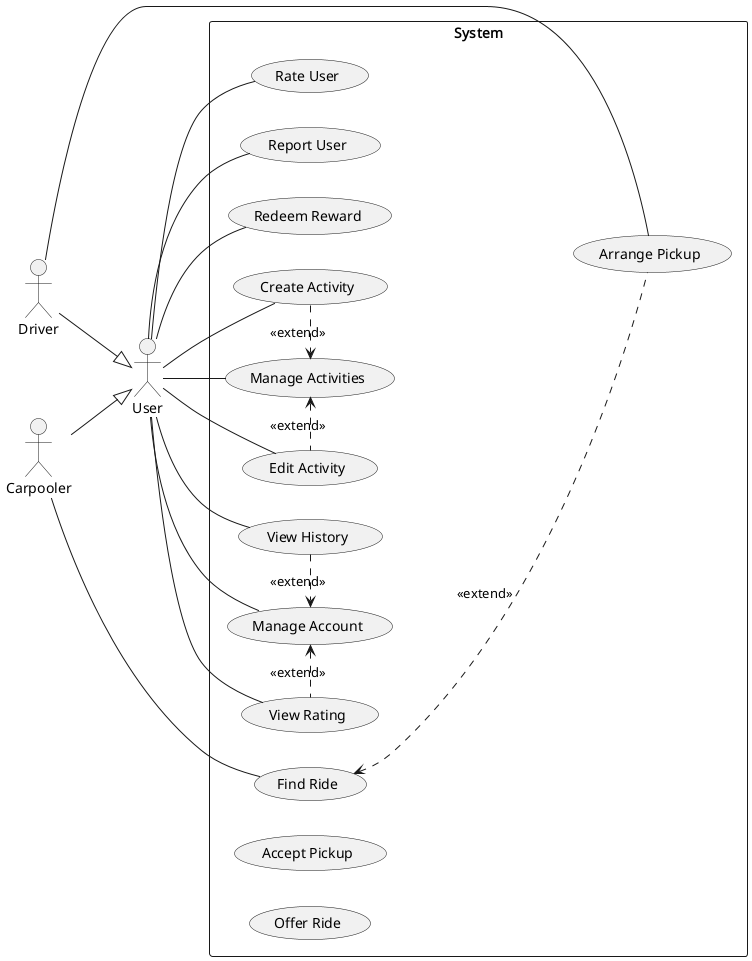
\includegraphics[width=0.8\textwidth]{uml/use-cases}
    \caption{Use Case Diagram}
\end{figure}

\end{document}
